\newpage
\begin{center}
  \textbf{\large 1. АНАЛИЗ ОТДЕЛЬНЫХ ПОСЛЕДОВАТЕЛЬНОСТЕЙ}
\end{center}
\refstepcounter{chapter}
\addcontentsline{toc}{chapter}{1. АНАЛИЗ ОТДЕЛЬНЫХ ПОСЛЕДОВАТЕЛЬНОСТЕЙ}

\section{Описание алгоритма PCA-Seq}

Метод главных компонент (PCA) \cite{pearson1901}~--- один из фундаментальных инструментов анализа данных, описанный Карлом Пирсоном в 1901-м году. Этот метод позволяет снижать размерность данных без значительной потери информации.

В 1940-х годах Кари Карунен и Мишель Лоэв предложили метод обработки одномерного числового ряда с использованием метода главных компонент (PCA-TS) \cite{karhunen, loeve}. Суть предложенного метода заключается в преобразовании исходного ряда в многомерный путем сдвига скользящего окна и последующем его разложении на ортогональные ряды методом главных компонент. В настоящее время этот метод чаще всего называют SSA (сингулярный спектральный анализ) \cite{Golyandina2013}.

В 2018-м году был разработан алгоритм PCA-Seq \cite{Efimov2020}, который распространяет метод PCA-TS на произвольную одномерную последовательность, и в качестве частного случая~--- на молекулярную последовательность (последовательность нуклеотидов или аминокислот).

Алгоритм использует идеи Джона Гауэра и разработанного им метода главных координат (PCoA) \cite{Gower1966}. В отличие от классического метода главных компонент, метод главных координат не требует наличия векторного представления объектов в исходном пространстве. Достаточно иметь матрицу евклидовых расстояний между ними, полученную любым способом.

Опишем алгоритм более детально.

Пусть дана произвольная последовательность длины $K$:

$$S = s_1s_2\ldots s_K.$$ 

Выберем два параметра алгоритма:
\begin{itemize}
  \item размер скользящего окна $W$,
  \item шаг скользящего окна $T$.
\end{itemize}

Пройдя скользящим окном по исходной последовательности, получим набор фрагментов (подстрок) равной длины:

\begin{itemize}
  \item $F_1 = s_1\ldots s_W$,
  \item $F_2 = s_{T+1}\ldots s_{T+W}$,
  \item $F_3 = s_{2T+1}\ldots s_{2T + W}$,
  \item $\ldots$
  \item $F_N = s_{K-W+1}\ldots s_K$.
\end{itemize}

В случае, если $K-W$ не кратно $T$, шаг между предпоследним и последним фрагментом может быть уменьшен, чтобы избежать потери информации о конце последовательности. В итоге мы получим $N~= \left\lceil\frac{K-W}{T}\right\rceil + 1$ фрагментов.

Пусть $d(x,y)$~--- некая метрика, определенная на множестве полученных фрагментов. Построим матрицу расстояний $D$ размерности $N\times N$, где $D_{ij}~= d(F_i, F_j)$.

Будем называть метрику $d$ и матрицу $D$ \textit{евклидовыми}, если существуют число $M$ и набор из $N$ точек $X = \{X_1,\ldots,X_N\}$ в пространстве размерности $M$, для которых выполнено:

$$D_{ij} = \sqrt{\sum_{k=1}^M \left(X_{ik} - X_{jk}\right)^2}, \; \forall i, j \in \{1,\ldots, N\}.$$

Гауэр показал \cite{Gower1966}, что если возвести элементы евклидовой матрицы $D$ в квадрат, затем применить к матрице двойное центрирование и умножение на $-\frac{1}{2}$, то будет получена матрица $XX^\top$. После применения к ней сингулярного разложения (SVD) получатся главные компоненты матрицы $X$.

В нашем случае это одновременно будут и главные компоненты фрагментов исходной последовательность $F_1,\ldots,F_N$.

Оценим вычислительную сложность полученного алгоритма. Для вычисления матрицы $D$ нам необходимо найти расстояние между каждой парой из $N$ фрагментов длины $W$. Если считать, что мы находим расстояние между двумя фрагментами за $O(W)$, то вычислительная сложность этой части алгоритма составит $O(N^2W)$. Далее мы ищем сингулярное разложение матрицы размерности $N\times N$, что занимает $O(N^3)$ времени. Итоговая сложность составляет $O(N^3 + N^2W) = O\left(\left(\frac{K-W}{T}\right)^3 + \left(\frac{K-W}{T}\right)^2W\right)$. Полагая $W \ll K$, можем считать сложность равной $O\left(\frac{K}{T}\right)^3$

Пространство главных компонент, полученных в результате работы алгоритма, будет отличаться в зависимости от того, какая метрика будет использована для вычисления матрицы расстояний. Авторы алгоритма PCA-Seq использовали в своей работе квадратный корень из $p$-дистанции (расстояния Хэмминга, деленного на длину последовательности). Первым этапом нашей работы было сравнение эффективности различных метрик в алгоритме PCA-Seq.

\section{Выбор метрик для расчета расстояний между фрагментами последовательностей}

В нашей работе мы решили рассмотреть метрики, основанные на частотных характеристиках фрагментов текста. Понятие частотной характеристики вводится, например, в работе В. Д. Гусева «Характеристики символьных последовательностей» \cite{gusev}.

Всякий фрагмент может быть представлен в виде последовательности частично перекрывающихся $L$-грамм, которые получаются путем сдвига на один или несколько символов скользящего окна длины $L$ вдоль фрагмента. Посчитав число повторений каждой из разновидностей $L$-грамм, деленное на суммарное количество $L$-грамм во фрагменте, получаем частотную характеристику фрагмента порядка $L$.

Пусть в исходной последовательности $S$ длины $K$ имеется $R$ различных $L$-грамм. Можно заметить, что $R\leqslant\min(K-L+1,\, T^L)$. Здесь $T^L$~--- мощность алфавита из $L$-грамм. В случае нуклеотидной последовательности $T=4$, в случае аминокислотной~--- $T = 20$. Тогда частотная характеристика каждого фрагмента исходной последовательности является вектором размера $R$.

\newpage
$$\vec{F} = (f_1,\ldots,f_R),$$
$$f_i \in [0,\,1],$$
$$\sum_i f_i = 1.$$

Размер $L$-граммы должен быть достаточно небольшим относительно размера фрагмента последовательности, чтобы одни и те же $L$-граммы встречались в разных фрагментах и при этом их частоты могли варьироваться.

Частотные характеристики для аминокислотных последовательностей известны \cite{Bhasin2004} в научной литературе, как:
\begin{itemize}
  \item Amino Acid Composition (AAC) при $L = 1$,
  \item Dipeptide Composition (DPC) при  $L = 2$,
  \item Tripeptide Composition (TPC) при  $L = 3$.
\end{itemize}

Пусть мы посчитали частотные характеристики для каждого из $N$ фрагментов исходной последовательности $S$. Пусть $f_{i,k}$~--- частота $L$-граммы $k$ во фрагменте $i$ ($i \in \{1,\ldots, N$\}, $k \in \{1, \ldots, R\}$).

Прежде всего, мы можем посчитать евклидовую метрику непосредственно в пространстве частотных характеристик. Обозначим эту метрику, как расстояние Пифагора. Слева от знака равенства здесь и далее будут указываться обозначения метрик, которые будут использоваться в следующих таблицах и графиках:

$$\text{pythagoras}(i,j) = \sqrt{\sum_k \left(f_{i,k} - f_{j,k}\right)^2}.$$

Далее рассмотрим вариацию расстояния Жаккара:

$$\text{jaccard}(i, j) = \sqrt{1-\frac{\sum_k \min(f_{i,k}, f_{j,k})}{\sum_k \max(f_{i,k}, f_{j,k})}}.$$

Эдвард Марчевский и Гуго Штейнгауз показали \cite{Marczewski1958}, что данная функция является метрикой. Ее евклидовость показали Джон Гауэр и Пьер Лежандр \cite{Gower1986}.

Дополнительно рассмотрим эту же метрику, но взяв из каждой частоты квадратный корень:

$$\text{jaccard\_with\_sqrt}(i, j) = \sqrt{1-\frac{\sum_k \min(\sqrt{f_{i,k}}, \sqrt{f_{j,k}})}{\sum_k \max(\sqrt{f_{i,k}}, \sqrt{f_{j,k}})}}.$$

Сумма квадратов таких элементов равна 1, поэтому их можно считать точкой единичной сферы. Луиджи Кавалли-Сфорца и Энтони Эдвардс ввели следующие две метрики \cite{CavalliSforza1967}. Первая из них равна длине хорды между двумя точками единичной сферы:

$$\text{cavalli\_sforza}(i,j) = \sqrt{\sum_k \left(\sqrt{f_{i,k}} - \sqrt{f_{j,k}}\right)^2}.$$

Вторая метрика равна длине дуги:

$$\text{arccosine}(i,j) = \left|\arccos\left(\sum_k\sqrt{f_{i,k}}\sqrt{f_{j,k}}\right)\right|.$$

Также рассмотрим метрику, которую мы назвали \textit{энтропийной}:

$$\text{entropy}(i,j) = \sqrt{\sum_k \left(f_{i,k}\ln f_{i,k} - f_{j,k}\ln f_{j,k}\right)^2}.$$

Очевидно, что она является евклидовой в пространстве, полученном отображением $x \mapsto x\ln x$.

Также мы взяли в рассмотрение две метрики, которые не основаны на частотных характеристиках. Первая из них~--- корень из $p$-дистанции, использованная авторами алгоритма PCA-Seq в своей работе:

$$\text{hamming}(i, j) = \sqrt{\frac{\sum_{x: F_i[x]\neq F_j[x]} 1}{W}}.$$

Здесь $F_i[x]$ --- символ, стоящий на позиции $x$ в $i$-м фрагменте.

В статье 2013 года было показано \cite{Efimov2013}, что эта метрика является евклидовой.

Вторая метрика, не основанная частотных характеристиках,~--- расстояние Левенштейна \cite{levenshtein1965}, которое определяется, как минимальное количество операций вставки, удаления и замены символа, необходимых для превращения одной последовательности символов в другую. Оно считается алгоритмом динамического программирования за $O(W^2)$.

Эта метрика не является евклидовой, а значит ее использование в исходном методе главных координат Гауэра некорректно. Некоторые главные компоненты, полученные с использованием этой метрики могут оказаться мнимыми. Но мы можем отфильтровать их, если вместо SVD будем использовать EVD (eigenvalue decomposition). В таком случае мнимые компоненты будут иметь отрицательные дисперсии.

\section{Сравнение эффективности метрик}

В качестве исходной молекулярной последовательности $S$, на которой производилось сравнение метрик, был взят митохондриальный геном человека (MT\_HUMAN), состоящий примерно из 16,5 тыс. пар нуклеотидов \cite{Anderson1981}. Эта последовательность имеет достаточно большой размер, и ее биологические и физические свойства хорошо изучены, что позволит в будущем на основе этой информации искать взаимосвязи с главными компонентами.

В качестве основного критерия эффективности мы использовали энтропию распределения дисперсий главных компонент, полученных в результате работы алгоритма. Низкое значение энтропии указывает на высокую эффективность полученных компонент.

Ниже будут показаны результаты работы алгоритма со следующими параметрами:
\begin{itemize}
  \item размер скользящего окна $W = 1000$,
  \item шаг скользящего окна $T = 100$,
  \item размер $L$-граммы $L = 3$.
\end{itemize}

На рисунке~\ref{dispersions} представлен график распределений дисперсии первых десяти главных компонент (в процентах), полученных для различных евклидовых метрик.

Метрики Пифагора, Кавалли-Сфорца и <<энтропийная>> продемонстрировали близкие распределения дисперсий. Метрики Жаккара показали более низкий результат: у них дисперсия первой главной компоненты приблизительно в два раза меньше, чем у других метрик. Показатели корня из $p$-дистанции и расстояния Левенштейна оказались значительно ниже, чем показатели метрик, основанных на частотных характеристиках.

В таблице~\ref{table-disp} представлены значения энтропии объясненных дисперсий для разных метрик. Расстояние Пифагора оказалось самым эффективным по этому критерию.

\begin{figure}[!t]
  \centering
  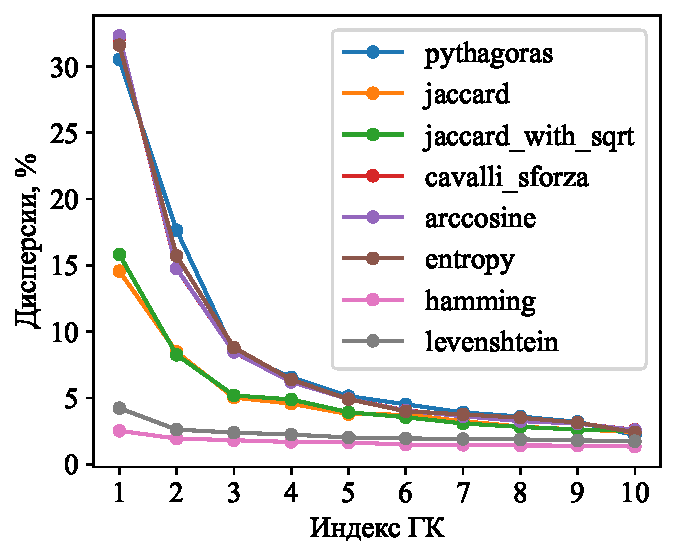
\includegraphics{dispersions.pdf}
  \caption{Распределения дисперсий первых десяти главных компонент для различных метрик}
  \label{dispersions}
\end{figure}

\begin{table}[h!]
  \centering{
    \begin{tabular}{|c|c|}
      \hline
      \textbf{Обозначение метрики} & \textbf{Энтропия распределения дисперсий}\\
      \hline
      pythagoras & 2.48\\
      entropy & 2.52\\
      arccosine	& 2.54\\
      cavalli\_sforza & 2.55\\
      jaccard\_with\_sqrt & 3.91\\
      jaccard & 3.98\\
      levenshtein & 4.63\\
      hamming & 4.88\\
      \hline
    \end{tabular}
  }
  \caption{Энтропия распределения дисперсий главных компонент для различных евклидовых метрик}
  \label{table-disp}
\end{table}

Рассмотрим главные компоненты MT\_HUMAN, полученные при помощи расстояния Пифагора. На рисунке~\ref{pc1-2} представлены значения первых двух главных компонент. Для удобства значения по оси $x$ приведены в соответствие с нумерацией нуклеотидов в исходной последовательности. Каждому фрагменту сопоставлен индекс нуклеотида, с которого он начинается.

\begin{figure}[!t]
  \centering
  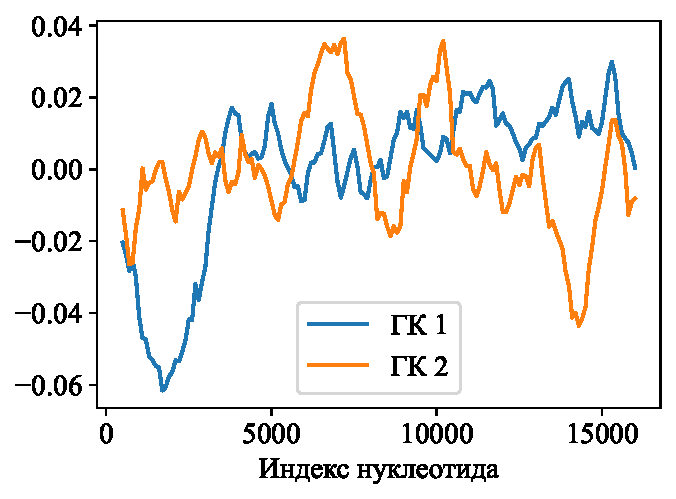
\includegraphics{pc1-2.pdf}
  \caption{Первые две главные компоненты MT\_HUMAN, полученные при помощи расстояния Пифагора}
  \label{pc1-2}
\end{figure}

Можно заметить, что первая компонента изначально резко убывает, затем возрастает и после этого не принимает больших отрицательных значений. У второй компоненты видны два скачка вверх в середине последовательности и один скачок вниз ближе к концу. На рисунке~\ref{trajectory} приведена фазовая траектория первых двух компонент, на которой эти особенности более наглядны.

\begin{figure}[!t]
  \centering
  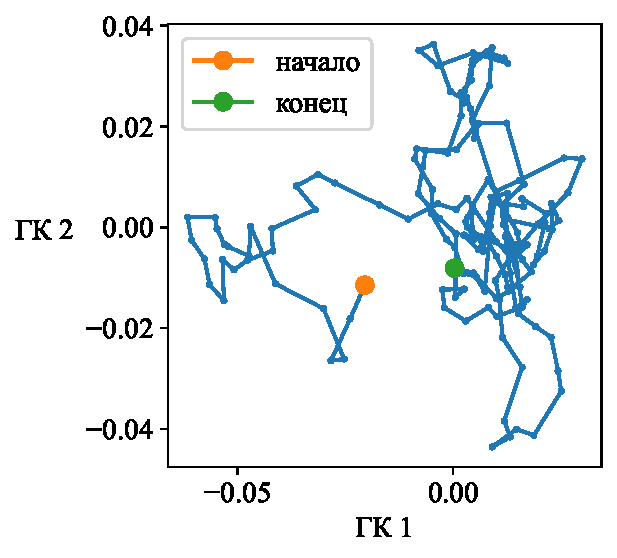
\includegraphics{trajectory.pdf}
  \caption{Фазовая траектория первых двух главных компонент MT\_HUMAN, полученных при помощи расстояния Пифагора}
  \label{trajectory}
\end{figure}

Исследовав корреляции между значениями главных компонент фрагментов последовательности и частотами $L$-грамм в этом фрагменте, мы обнаружили, что наибольший по модулю коэффициент корреляции у первой главной компоненты с триплетом AAG ($r = -0.932$), который кодирует аминокислоту лизин. На рисунке~\ref{corr-AAG} представлены графики коррелирующих величин. Так как коэффициент корреляции отрицательный, для наглядности взяты противоположные по знаку значения главной компоненты.

\begin{figure}[!t]
  \centering
  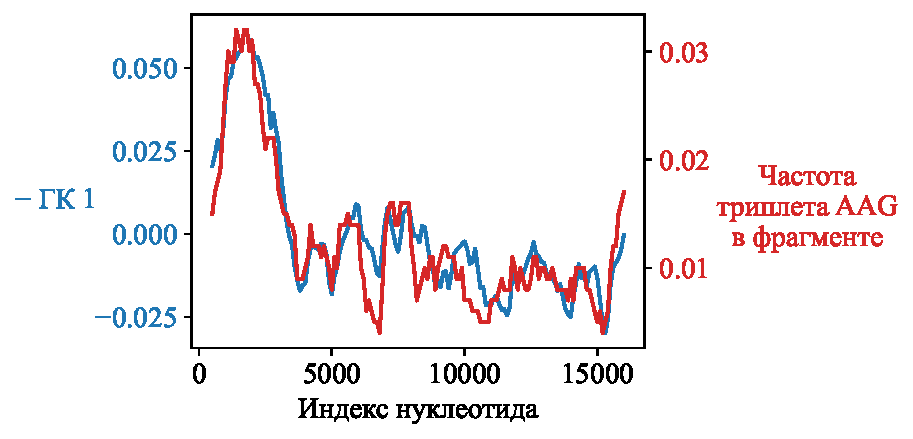
\includegraphics{corr-AAG.pdf}
  \caption{Графики первой ГК, умноженной на $-1$, и частот триплета AAG в фрагментах последовательности}
  \label{corr-AAG}
\end{figure}

\section{Исследование чувствительности метода к фрагментам интронов и экзонов}

Одно из ключевых свойств фрагмента последовательности ДНК~--- это его принадлежность интрону или экзону. Интрон~--- участок ДНК, удаляемый из первичного транскрипта и отсутствующий в зрелой РНК. Одним из этапов нашей работы было тестирование алгоритма PCA-Seq на чувствительность к участкам интронов и экзонов в последовательностях ДНК.

Для каждого фрагмента последовательности мы считали, какая его часть находится в интронах. Далее мы искали главные компоненты, имеющие высокий коэффициент корреляции с полученной величиной.

В митохондриальном геноме человека интроны отсутствуют, а в ядерном геноме суммарная длина участков интронов значительно превышает суммарную длину участков экзонов, поэтому для поставленной задачи геномные последовательности человека не подходят. Необходим организм, в ДНК которого соотношение интронов и экзонов примерно одинаково.

В качестве объекта исследования мы взяли ген F53H8.3 почвенной нематоды (Caenorhabditis elegans) из базы WormBase \cite{Harris2003}. В этом гене участки интронов занимают 61\% последовательности. Длина последовательности~--- 4167 нуклеотидов.

Высокий коэффициент корреляции с долей интронов во фрагменте был найден у второй главной компоненты, полученной со следующими параметрами алгоритма:

\begin{itemize}
  \item размер скользящего окна $W = 200$,
  \item шаг скользящего окна $T = 40$,
  \item метрика --- расстояние Пифагора между частотными характеристиками,
  \item размер $L$-граммы $L = 5$.
\end{itemize}

Коэффициент корреляции оказался равен 0.78. На рисунке~\ref{exons} представлены графики полученной компоненты и долей интронов внутри фрагментов последовательности.

\begin{figure}[!t]
  \centering
  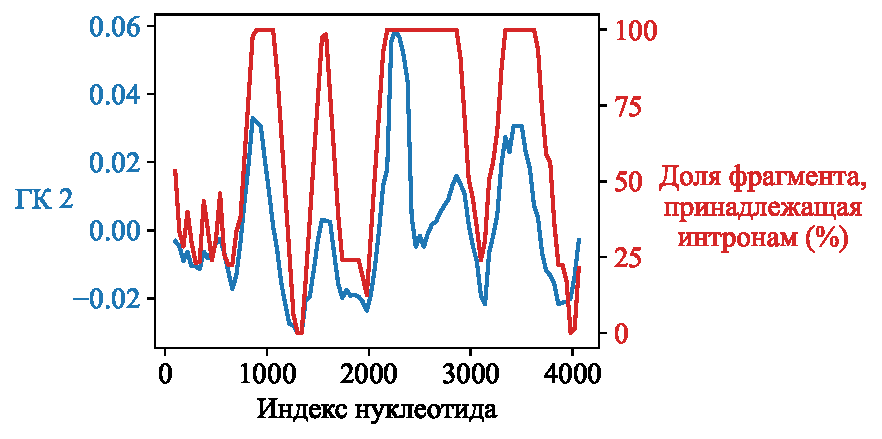
\includegraphics{exons.pdf}
  \caption{Графики второй ГК и долей интронов внутри фрагментов последовательности}
  \label{exons}
\end{figure}

Из полученных результатов мы можем сделать вывод, что алгоритм может выявлять скрытые биологические свойства молекулярных последовательностей, явным образом ему не передаваемые, на основе только цепочки нуклеотидов или аминокислот.
